%%%%%%%%%%%%%%%%%%%%%%%%%%%%%%%%%%%%%%%%%%%%%%%%%%%%%%%%%%%%%%%%%%%%%%%%%%%%%%%%%%%%%%%%%%%%%%%%%%%%%%%%%%%%%%%%%%%%%%%%%%%%%%%%%%%%%%%%%%%%%%%%%%%%%%%%%%%%%%%%%%%
% Written By Michael Brodskiy
% Class: Fundamentals of Electronics
% Professor: I. Salama
%%%%%%%%%%%%%%%%%%%%%%%%%%%%%%%%%%%%%%%%%%%%%%%%%%%%%%%%%%%%%%%%%%%%%%%%%%%%%%%%%%%%%%%%%%%%%%%%%%%%%%%%%%%%%%%%%%%%%%%%%%%%%%%%%%%%%%%%%%%%%%%%%%%%%%%%%%%%%%%%%%%

\include{Includes.tex}

\title{Pre-Lab 2}
\date{\today}
\author{Michael Brodskiy\\ \small Professor: M. Onabajo}

\begin{document}

\maketitle

\begin{enumerate}

  \item

    Using the equation:

    $$i=I_s\left( e^{v/(nV_T)}-1 \right)$$

    and the given measurements, we may write:

    $$10^{-3}=I_s\left( e^{.62/(n.025)}-1 \right)$$
    $$10^{-2}=I_s\left( e^{.69/(n.025)}-1 \right)$$

    Since the exponential is greater than 1, we may simplify to:

    $$\frac{10^{-3}}{e^{24.8/n}}=I_s$$
    $$\frac{10^{-2}}{e^{27.6/n}}=I_s$$

    $$I_s=.001e^{-\frac{24.8}{n}}$$
    $$I_s=.01e^{-\frac{27.6}{n}}$$

    We can combine the two equations to solve for $n$ and $I_s$:

    $$.001e^{-\frac{24.8}{n}}=.01e^{-\frac{27.6}{n}}$$
    $$e^{-\frac{24.8}{n}}=10e^{-\frac{27.6}{n}}$$
    $$e^{\frac{27.6-24.8}{n}}=10$$
    $$\frac{27.6-24.8}{n}=\ln(10)$$
    $$n=\frac{2.8}{\ln(10)}$$
    $$\boxed{n=1.216}$$

    We then plug this into the earlier equations to find $I_s$:

    $$I_s=.001e^{-24.8/1.216}$$
    $$\boxed{I_s=1.3889\cdot10^{-12}[\si{\ampere}]}$$

    We can verify by using the second equation for $I_s$:

    $$I_s=.01e^{-27.6/1.216}$$
    $$\boxed{I_s=1.3889\cdot10^{-12}[\si{\ampere}]}$$

    It is difficult to measure the current in a reverse bias mode, however, because the diode may reach breakdown voltage by increasing the reverse voltage.

  \item Read through, no questions \textcolor{green}{\checkmark}

  \item Taking the forward voltage of the LEDs as $.2[\si{\volt}]$, and the input as $8[\si{\volt}]$, we can make some relevant calculations, assuming each LED will form a ``branch'' consisting of a resistor and the LED itself. First, using the maximum power, we can calculate the maximum current, starting with the first (red) LED to turn on:

    $$I_{max}=\frac{6\cdot10^{-2}}{.2}=.3[\si{\ampere}]$$

    Now, we find the resistance value:

    $$R_{red}=\frac{8-.2}{.3}=26[\si{\ohm}]$$

    We then cascade this with the next LED to turn on (yellow), and calculate (using the Zener rating):

    $$I_{max}^2=\frac{1}{8}=.125[\si{\amp}]$$

    Summing this with the current flowing through $R_{red}$, we get:

    $$I_{yel}=.425[\si{\amp}]$$

    From which we derive a resistor value:

    $$R_{yel}=\frac{17-8}{.425}=21.176[\si{\ohm}]$$

    Repeating a similar process for green, we find:

    $$R_{grn}=\frac{24-8}{.425}=37.647[\si{\ohm}]$$

    We combine the cascade, along with a $26[\si{\ohm}]$ series resistor to get:

    \begin{figure}[H]
      \centering
      \tikzset{every picture/.style={line width=0.75pt}} %set default line width to 0.75pt        

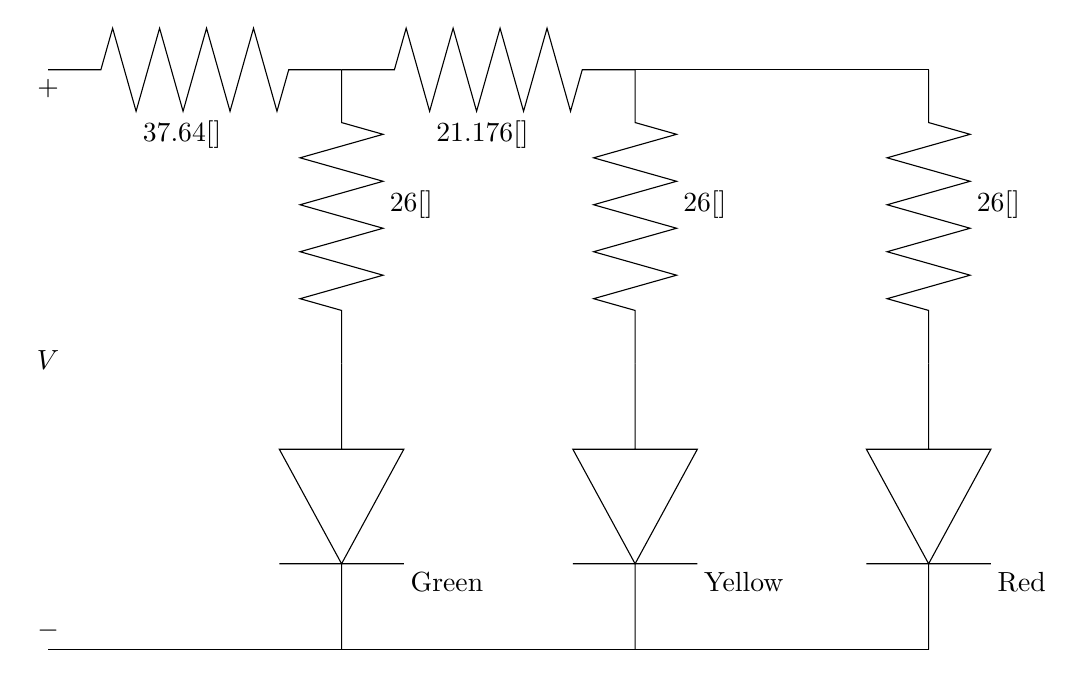
\begin{tikzpicture}[x=0.75pt,y=0.75pt,yscale=-1,xscale=1]
%uncomment if require: \path (0,757); %set diagram left start at 0, and has height of 757

%Shape: Diode [id:dp9916766022166023] 
\draw   (567,293.4) -- (537,348.6) -- (507,293.4) -- (567,293.4) -- cycle (537,252) -- (537,293.4) (567,348.6) -- (507,348.6) (537,348.6) -- (537,390) ;
%Shape: Diode [id:dp47724199606317685] 
\draw   (425.58,293.4) -- (395.58,348.6) -- (365.58,293.4) -- (425.58,293.4) -- cycle (395.58,252) -- (395.58,293.4) (425.58,348.6) -- (365.58,348.6) (395.58,348.6) -- (395.58,390) ;
%Straight Lines [id:da43394379079125567] 
\draw    (537,390) -- (395.58,390) ;
%Shape: Resistor [id:dp7260924477087448] 
\draw   (537,110.58) -- (537,136.03) -- (557,141.69) -- (517,153.01) -- (557,164.32) -- (517,175.63) -- (557,186.95) -- (517,198.26) -- (557,209.57) -- (517,220.89) -- (537,226.54) -- (537,252) ;
%Shape: Resistor [id:dp09973725738727013] 
\draw   (395.58,110.58) -- (395.58,136.03) -- (415.58,141.69) -- (375.58,153.01) -- (415.58,164.32) -- (375.58,175.63) -- (415.58,186.95) -- (375.58,198.26) -- (415.58,209.57) -- (375.58,220.89) -- (395.58,226.54) -- (395.58,252) ;
%Straight Lines [id:da9934104451259984] 
\draw    (537,110.58) -- (395.58,110.58) ;
%Shape: Resistor [id:dp5223648498783691] 
\draw   (254.16,110.58) -- (279.61,110.58) -- (285.27,90.58) -- (296.58,130.58) -- (307.9,90.58) -- (319.21,130.58) -- (330.52,90.58) -- (341.84,130.58) -- (353.15,90.58) -- (364.47,130.58) -- (370.12,110.58) -- (395.58,110.58) ;
%Shape: Diode [id:dp30609907031657446] 
\draw   (284.16,293.4) -- (254.16,348.6) -- (224.16,293.4) -- (284.16,293.4) -- cycle (254.16,252) -- (254.16,293.4) (284.16,348.6) -- (224.16,348.6) (254.16,348.6) -- (254.16,390) ;
%Shape: Resistor [id:dp3336013122238709] 
\draw   (254.16,110.58) -- (254.16,136.03) -- (274.16,141.69) -- (234.16,153.01) -- (274.16,164.32) -- (234.16,175.63) -- (274.16,186.95) -- (234.16,198.26) -- (274.16,209.57) -- (234.16,220.89) -- (254.16,226.54) -- (254.16,252) ;
%Straight Lines [id:da4142874846716025] 
\draw    (395.58,390) -- (254.16,390) ;
%Shape: Resistor [id:dp416533824669727] 
\draw   (112.74,110.58) -- (138.19,110.58) -- (143.85,90.58) -- (155.16,130.58) -- (166.48,90.58) -- (177.79,130.58) -- (189.1,90.58) -- (200.42,130.58) -- (211.73,90.58) -- (223.04,130.58) -- (228.7,110.58) -- (254.16,110.58) ;
%Straight Lines [id:da6359356780714503] 
\draw    (254.16,390) -- (112.74,390) ;

% Text Node
\draw (559,167.72) node [anchor=north west][inner sep=0.75pt]    {$26[ \si{\ohm}]$};
% Text Node
\draw (417.58,167.72) node [anchor=north west][inner sep=0.75pt]    {$26[ \si{\ohm}]$};
% Text Node
\draw (276.16,167.72) node [anchor=north west][inner sep=0.75pt]    {$26[ \si{\ohm}]$};
% Text Node
\draw (298.58,133.98) node [anchor=north west][inner sep=0.75pt]    {$21.176[ \si{\ohm}]$};
% Text Node
\draw (157.16,133.98) node [anchor=north west][inner sep=0.75pt]    {$37.64[ \si{\ohm}]$};
% Text Node
\draw (569,351.6) node [anchor=north west][inner sep=0.75pt]   [align=left] {Red};
% Text Node
\draw (427.58,351.6) node [anchor=north west][inner sep=0.75pt]   [align=left] {Yellow};
% Text Node
\draw (286.16,351.6) node [anchor=north west][inner sep=0.75pt]   [align=left] {Green};
% Text Node
\draw (112.74,113.98) node [anchor=north] [inner sep=0.75pt]    {$+$};
% Text Node
\draw (112.74,386.6) node [anchor=south] [inner sep=0.75pt]    {$-$};
% Text Node
\draw (112.74,250.29) node    {$V$};


\end{tikzpicture}

      \caption{LED Configuration}
      \label{fig:1}
    \end{figure}

    This, however, is not the final step, as we need to add an additional diode in tandem with a resistor to maintain a safe operating range for the LEDs. Thus, our final circuit becomes:

    \begin{figure}[H]
      \centering
      \tikzset{every picture/.style={line width=0.75pt}} %set default line width to 0.75pt        

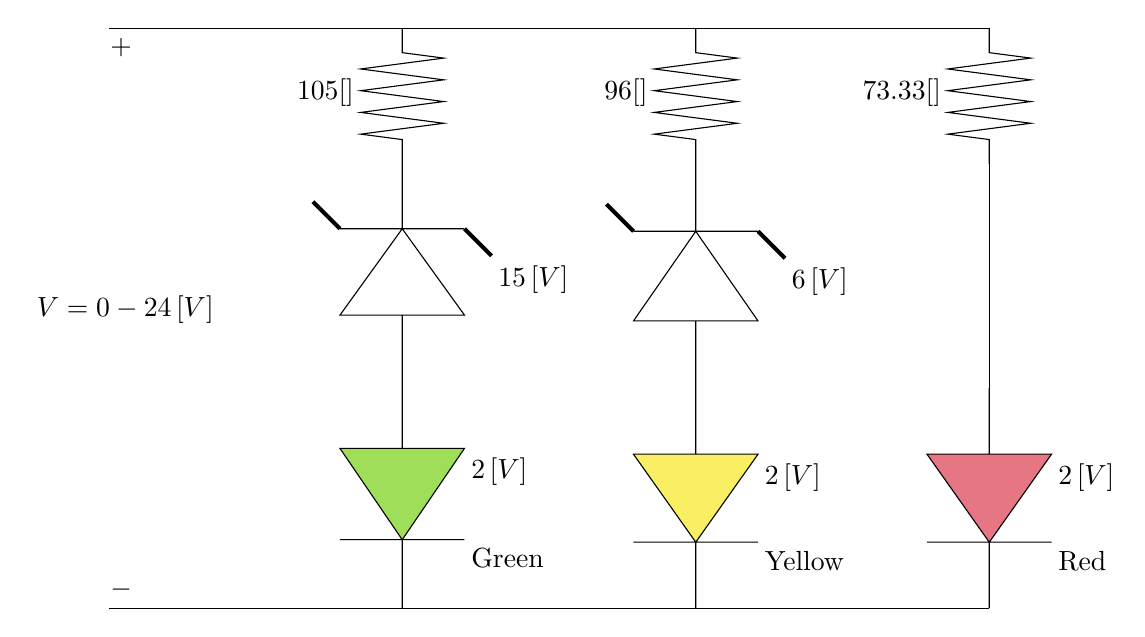
\begin{tikzpicture}[x=0.75pt,y=0.75pt,yscale=-1,xscale=1]
%uncomment if require: \path (0,412); %set diagram left start at 0, and has height of 412

%Shape: Diode [id:dp9916766022166023] 
\draw  [fill={rgb, 255:red, 208; green, 2; blue, 27 }  ,fill opacity=0.54 ] (611,315.8) -- (581,358.2) -- (551,315.8) -- (611,315.8) -- cycle (581,284) -- (581,315.8) (611,358.2) -- (551,358.2) (581,358.2) -- (581,390) ;
%Shape: Diode [id:dp47724199606317685] 
\draw  [fill={rgb, 255:red, 248; green, 231; blue, 28 }  ,fill opacity=0.69 ] (469.58,315.8) -- (439.58,358.2) -- (409.58,315.8) -- (469.58,315.8) -- cycle (439.58,284) -- (439.58,315.8) (469.58,358.2) -- (409.58,358.2) (439.58,358.2) -- (439.58,390) ;
%Straight Lines [id:da43394379079125567] 
\draw    (581,390) -- (439.58,390) ;
%Shape: Resistor [id:dp09973725738727013] 
\draw   (439.58,110.58) -- (439.58,122.35) -- (459.58,124.97) -- (419.58,130.21) -- (459.58,135.44) -- (419.58,140.67) -- (459.58,145.91) -- (419.58,151.14) -- (459.58,156.37) -- (419.58,161.61) -- (439.58,164.22) -- (439.58,176) ;
%Straight Lines [id:da9934104451259984] 
\draw    (581,110.58) -- (439.58,110.58) ;
%Shape: Diode [id:dp30609907031657446] 
\draw  [fill={rgb, 255:red, 126; green, 211; blue, 33 }  ,fill opacity=0.75 ] (328.16,313) -- (298.16,357) -- (268.16,313) -- (328.16,313) -- cycle (298.16,280) -- (298.16,313) (328.16,357) -- (268.16,357) (298.16,357) -- (298.16,390) ;
%Shape: Resistor [id:dp3336013122238709] 
\draw   (298.16,110.58) -- (298.16,122.35) -- (318.16,124.97) -- (278.16,130.21) -- (318.16,135.44) -- (278.16,140.67) -- (318.16,145.91) -- (278.16,151.14) -- (318.16,156.37) -- (278.16,161.61) -- (298.16,164.22) -- (298.16,176) ;
%Straight Lines [id:da4142874846716025] 
\draw    (439.58,390) -- (298.16,390) ;
%Straight Lines [id:da6359356780714503] 
\draw    (298.16,390) -- (156.74,390) ;
%Straight Lines [id:da792670839882941] 
\draw    (439.58,110.58) -- (298.16,110.58) ;
%Straight Lines [id:da5542473757631496] 
\draw    (298.16,110.58) -- (156.74,110.58) ;
%Shape: Diode [id:dp6229217229836789] 
\draw   (268.16,248.8) -- (298.16,207.2) -- (328.16,248.8) -- (268.16,248.8) -- cycle (298.16,280) -- (298.16,248.8) (268.16,207.2) -- (328.16,207.2) (298.16,207.2) -- (298.16,176) ;
%Shape: Diode [id:dp2807840415796292] 
\draw   (409.58,251.6) -- (439.58,208.4) -- (469.58,251.6) -- (409.58,251.6) -- cycle (439.58,284) -- (439.58,251.6) (409.58,208.4) -- (469.58,208.4) (439.58,208.4) -- (439.58,176) ;
%Straight Lines [id:da9880872033365566] 
\draw [line width=1.5]    (255.13,194.17) -- (268.16,207.2) ;
%Straight Lines [id:da4671561501686561] 
\draw [line width=1.5]    (328.16,207.2) -- (341.18,220.23) ;
%Straight Lines [id:da7936008436502483] 
\draw [line width=1.5]    (396.55,195.37) -- (409.58,208.4) ;
%Straight Lines [id:da3769618486887958] 
\draw [line width=1.5]    (469.58,208.4) -- (482.6,221.43) ;
%Straight Lines [id:da15712761589306246] 
\draw    (581,284) -- (581,176) ;
%Shape: Resistor [id:dp44020554709517357] 
\draw   (581,110.58) -- (581,122.35) -- (601,124.97) -- (561,130.21) -- (601,135.44) -- (561,140.67) -- (601,145.91) -- (561,151.14) -- (601,156.37) -- (561,161.61) -- (581,164.22) -- (581,176) ;

% Text Node
\draw (613,361.2) node [anchor=north west][inner sep=0.75pt]   [align=left] {Red};
% Text Node
\draw (471.58,361.2) node [anchor=north west][inner sep=0.75pt]   [align=left] {Yellow};
% Text Node
\draw (330.16,360) node [anchor=north west][inner sep=0.75pt]   [align=left] {Green};
% Text Node
\draw (162.74,113.98) node [anchor=north] [inner sep=0.75pt]    {$+$};
% Text Node
\draw (162.74,386.6) node [anchor=south] [inner sep=0.75pt]    {$-$};
% Text Node
\draw (164.74,246.29) node    {$V=0-24\left[\text{V}\right]$};
% Text Node
\draw (484.6,224.83) node [anchor=north west][inner sep=0.75pt]    {$6\left[\text{V}\right]$};
% Text Node
\draw (471.58,319.2) node [anchor=north west][inner sep=0.75pt]    {$2\left[\text{V}\right]$};
% Text Node
\draw (613,319.2) node [anchor=north west][inner sep=0.75pt]    {$2\left[\text{V}\right]$};
% Text Node
\draw (330.16,316.4) node [anchor=north west][inner sep=0.75pt]    {$2\left[\text{V}\right]$};
% Text Node
\draw (343.18,223.63) node [anchor=north west][inner sep=0.75pt]    {$15\left[\text{V}\right]$};
% Text Node
\draw (559,133.61) node [anchor=north east] [inner sep=0.75pt]    {$73.33[ \si{\ohm}]$};
% Text Node
\draw (417.58,133.61) node [anchor=north east] [inner sep=0.75pt]    {$96[ \si{\ohm}]$};
% Text Node
\draw (276.16,133.61) node [anchor=north east] [inner sep=0.75pt]    {$105[ \si{\ohm}]$};


\end{tikzpicture}

      \caption{Final Configuration}
      \label{fig:2}
    \end{figure}

\end{enumerate}

\end{document}

